\chapter{Kekontinuan dan Kekontinuan Seragam}

Sebuah program memotret $f(x)=1/x$ pada kisi titik berjarak $10^{-4}$ di dalam
$(0,1]$. Di sekitar $x=10^{-4}$ dua titik bertetangga, yaitu $10^{-4}$ dan
$2\times 10^{-4}$, memberi keluaran $10000$ dan $5000$; selisihnya $5000$. Di sekitar
$x=1$ dua titik bertetangga memberi $1$ dan $1.0001$; selisihnya sekitar $10^{-4}$.
Fungsi yang sama, jarak kisi yang sama, dua selisih yang berbeda tujuh pangkat.

Pertanyaan yang muncul bukan ``apakah $1/x$ kontinu'', sebab jawabannya ya di setiap
titik $(0,1]$. Pertanyaannya lain: berapa jarak kisi yang harus dipakai supaya
\emph{seluruh} keluaran pada interval itu bertahan di dalam satu toleransi? Untuk
toleransi $10^{-2}$, titik $x=1$ hanya menuntut jarak di bawah
$9.901\times 10^{-3}$, sedangkan titik $x=10^{-4}$ menuntut jarak di bawah
$1.000\times 10^{-10}$. Nisbah kedua tuntutan itu $9.9\times 10^{7}$. Tidak ada satu
jarak pun yang melayani keduanya, dan itu bukan cacat program.

Bab 4 memberi limit barisan, Bab 3 memberi supremum, dan keduanya belum cukup: limit
fungsi membandingkan $f$ dengan satu bilangan tetap, sehingga ia tidak dapat
membandingkan dua keluaran dari dua masukan berdekatan. Yang dibutuhkan adalah satu
ambang untuk seluruh himpunan, beserta cara membuktikan bahwa ambang itu ada. Bab ini
menyusun alat tersebut, dari definisi $\varepsilon$-$\delta$ sampai himpunan kompak dan
kelas fungsi Lipschitz, lalu menutup dengan fungsi yang kontinu di satu titik saja.

\begin{untukanak}
Bayangkan tangga darurat dengan anak tangga yang makin ke atas makin tinggi. Di
bagian bawah, satu langkah selebar telapak kaki menaikkan kita sedikit. Di bagian
atas, langkah selebar itu menaikkan kita sejengkal, lalu sehasta, lalu hampir
setinggi badan. Kakak kita berdiri di samping dan menanyakan satu hal: berapa lebar
langkah yang aman untuk seluruh tangga? Jawaban jujur untuk tangga seperti itu tidak
ada. Lebar yang aman di bawah terlalu lebar di atas, dan lebar yang aman di atas
membuat kita merangkak di bawah.

Sekarang pertanyaan yang membuat penasaran. Apakah semua tangga begitu? Ada tangga
yang anak tangganya tetap, dan ada tangga yang anak tangganya berubah tetapi tidak
pernah melewati batas tertentu. Untuk tangga jenis kedua, satu lebar langkah berlaku
dari bawah sampai atas. Bedanya bukan pada tinggi tangga, melainkan pada seberapa
curam kemiringannya berubah.

Hal yang sama terjadi pada grafik fungsi. Ada grafik yang bisa dijaga dengan satu
aturan jarak di seluruh daerahnya, ada yang menuntut aturan berbeda di setiap titik.
Di bab ini kita akan tahu mengapa perbedaan itu bisa dibuktikan dengan pasti, dan
mengapa daerah yang tertutup dan terbatas selalu termasuk jenis yang pertama.
\end{untukanak}

\section{Limit fungsi dan ambang delta}
\tingkat{dasar}

Kata ``mendekati'' tidak dapat dipakai sebagai definisi, karena setiap orang boleh
mengartikannya berbeda. Yang dapat dipakai adalah taruhan: berapa pun ketelitian yang
diminta, keluaran akan masuk ke dalam batas ketelitian itu asalkan masukannya cukup
dekat. Kalimat sehari-harinya: kita memasang jendela sempit di sekitar $L$, dan
menuntut $f$ masuk ke jendela itu untuk semua $x$ yang cukup dekat ke $c$.

\kamus{limit fungsi}{functional limit}{janji bahwa keluaran bisa dipaksa masuk ke
jendela sempit asalkan masukan cukup dekat dengan pintunya}

Sebelum definisinya, satu istilah teknis diperlukan. Titik $c$ disebut \emph{titik
limit}\index{titik limit} himpunan $A$ bila setiap interval terbuka di sekitar $c$
memuat titik $A$ selain $c$. Tanpa syarat itu, definisi limit menjadi hampa di titik
terpencil.

\begin{definisi}[Limit fungsi]
\index{limit fungsi}
Misalkan $A\subseteq\mathbb{R}$, $c$ titik limit $A$, dan $f\colon A\to\mathbb{R}$.
Kita tulis $\lim_{x\to c}f(x)=L$ bila untuk setiap $\varepsilon>0$ terdapat
$\delta>0$ sehingga untuk setiap $x\in A$ dengan $0<|x-c|<\delta$ berlaku
$|f(x)-L|<\varepsilon$.
\end{definisi}

Dua hal mudah terlewat. Pertama, syarat $0<|x-c|$ berarti nilai $f$ di $c$ tidak ikut
dihitung; fungsi boleh tidak terdefinisi di $c$ dan limitnya tetap ada. Kedua, urutan
kuantor: $\delta$ boleh bergantung pada $\varepsilon$, tetapi tidak pada $x$. Pada
bagian tentang kekontinuan seragam, kebebasan itulah yang diperdebatkan.

Definisi ini alat memeriksa, bukan resep mencari $\delta$; $\delta$ dicari dengan
bekerja mundur dari $|f(x)-L|$. Untuk
\[
f(x)=\frac{x^{2}-1}{x-1}\quad (x\neq 1),\qquad L=2,
\]
aljabar memberi $f(x)=x+1$, sehingga $|f(x)-2|=|x-1|$. Jadi $\delta=\varepsilon$
bekerja. Untuk $\varepsilon=10^{-2}$ ambil $\delta=10^{-2}$: pada $x=1+10^{-2}$
selisihnya tepat $10^{-2}$, dan itu \emph{belum} memenuhi syarat ketat; pada
$x=1+5\times10^{-3}$ selisihnya $5\times10^{-3}$. Karena itu $\delta=\varepsilon/2$ adalah pilihan
yang aman, dan $\delta=\varepsilon$ adalah pilihan paling murah yang batasnya tidak
pernah dicapai dari dalam.

Satu hal yang wajar dituntut dari limit adalah ketunggalannya: sebuah fungsi tidak
dapat berhenti di dua tempat berbeda sekaligus.

\begin{teorema}[Ketunggalan limit]
\index{limit fungsi}
Jika $\lim_{x\to c}f(x)=L_{1}$ dan $\lim_{x\to c}f(x)=L_{2}$, maka $L_{1}=L_{2}$.
\end{teorema}

\begin{proof}[Bukti]
Andaikan $L_{1}\neq L_{2}$ dan tetapkan $\varepsilon=|L_{1}-L_{2}|/2>0$. Ada
$\delta_{1}>0$ sehingga $0<|x-c|<\delta_{1}$ memberi $|f(x)-L_{1}|<\varepsilon$, dan
ada $\delta_{2}>0$ sehingga $0<|x-c|<\delta_{2}$ memberi $|f(x)-L_{2}|<\varepsilon$.
Ambil $x$ dengan $0<|x-c|<\min(\delta_{1},\delta_{2})$; titik seperti itu ada karena
$c$ titik limit. Maka
\[
|L_{1}-L_{2}|\le|L_{1}-f(x)|+|f(x)-L_{2}|<2\varepsilon=|L_{1}-L_{2}|,
\]
suatu kemustahilan. Jadi $L_{1}=L_{2}$.
\end{proof}

Kita juga memakai satu jembatan yang tidak dibuktikan di sini: limit fungsi ada dan
bernilai $L$ tepat ketika setiap barisan $x_{n}\to c$ dengan $x_{n}\neq c$ memenuhi
$f(x_{n})\to L$. Namanya kriteria barisan; buktinya ada di Abbott, \emph{Understanding
Analysis}, Bab 4 bagian Functional Limits, dan di Rudin, \emph{Principles of
Mathematical Analysis}, Bab 4 bagian Continuous Functions. Jembatan itu yang membuat
barisan dari Bab 4 dapat dipakai membongkar limit yang tidak ada. Untuk $g(x)=x/|x|$,
barisan $1/n$ memberi $g\to 1$ sedangkan $-1/n$ memberi $g\to -1$; dua limit berbeda,
jadi $\lim_{x\to 0}g(x)$ tidak ada. Pola itu dipakai lagi pada kekontinuan seragam,
dengan dua barisan yang jaraknya menuju nol.

\section{Kekontinuan dan sifat aljabarnya}
\tingkat{menengah}

Limit membandingkan $f$ dengan bilangan $L$ yang berdiri sendiri. Kekontinuan meminta
sesuatu yang lebih ketat: bilangan itu haruslah nilai fungsi di titiknya. Kalimat
sehari-harinya: grafik tidak melompat di titik itu, dan nilainya di titik itu memang
nilai yang didekati dari kiri dan kanan.

\kamus{kontinu}{continuous}{grafik yang dapat digambar tanpa mengangkat pena di
titik itu}

\begin{definisi}[Kekontinuan di satu titik]
\index{kontinu}
Misalkan $f\colon A\to\mathbb{R}$ dan $c\in A$. Fungsi $f$ \emph{kontinu di $c$} bila
untuk setiap $\varepsilon>0$ terdapat $\delta>0$ sehingga untuk setiap $x\in A$
dengan $|x-c|<\delta$ berlaku $|f(x)-f(c)|<\varepsilon$. Fungsi disebut kontinu pada
$A$ bila ia kontinu di setiap titik $A$.
\end{definisi}

Perhatikan bahwa $x=c$ kini diizinkan, dan yang diminta bukan sekadar limitnya ada,
melainkan limitnya sama dengan nilai fungsinya. Karena itu kekontinuan bersifat
lokal: ia hanya berbicara tentang perilaku $f$ di sekitar satu titik.

Untuk $f(x)=x^{2}$ di $c=2$ dan $\varepsilon>0$ berlaku $|x^{2}-4|=|x-2|\,|x+2|$, dan
bila $|x-2|<1$ maka $|x+2|<5$. Jadi $\delta=\min(1,\varepsilon/5)$ bekerja, sedangkan
$\delta$ terbesar yang masih sah adalah akar positif dari $\delta(4+\delta)=\varepsilon$,
yaitu $2.49984376953\times10^{-4}$ untuk $\varepsilon=10^{-3}$. Selisih kedua angka itu
adalah harga keamanan yang dibayar karena tidak mau menghitung akar.
Gambar~\ref{fig:epsdelta} memperlihatkan kedua ambang itu untuk $\varepsilon=1$.

\begin{figure}[htbp]
\centering
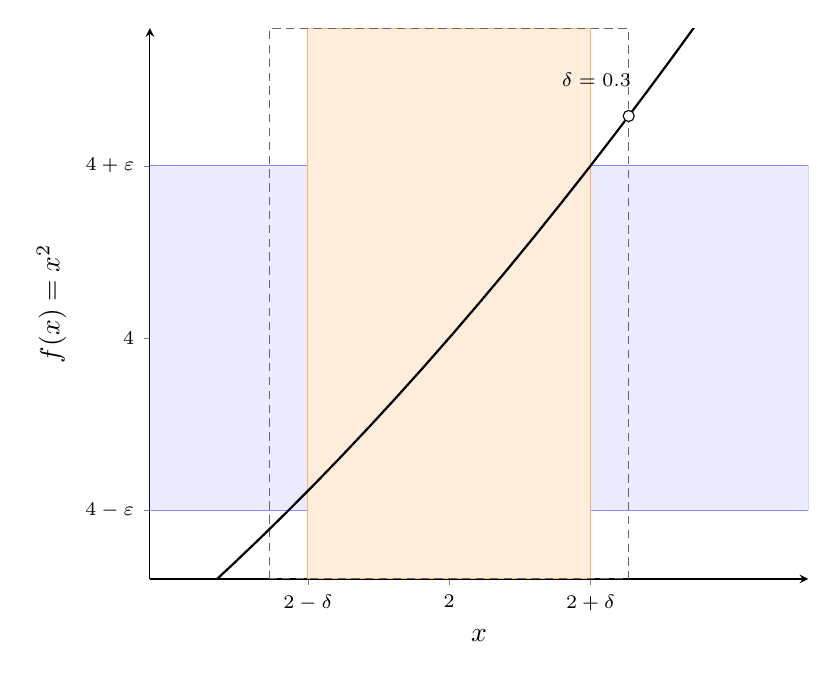
\begin{tikzpicture}
\begin{axis}[width=0.82\linewidth,
  axis lines=left,xmin=1.5,xmax=2.6,ymin=2.6,ymax=5.8,
  xlabel={$x$},ylabel={$f(x)=x^{2}$},
  xtick={1.7639,2,2.2361},xticklabels={$2-\delta$,$2$,$2+\delta$},
  ytick={3,4,5},yticklabels={$4-\varepsilon$,$4$,$4+\varepsilon$},
  tick label style={font=\scriptsize}]
\fill[blue!8,draw=blue!45] (1.5,3) rectangle (2.6,5);
\fill[orange!14,draw=orange!60] (1.7639,2.6) rectangle (2.2361,5.8);
\draw[densely dashed,black!60] (1.7,2.6) rectangle (2.3,5.8);
\addplot[thick,domain=1.5:2.6] {x^2};
\draw[fill=white] (2.3,5.29) circle (2pt);
\node[font=\scriptsize,anchor=east] at (2.32,5.5) {$\delta=0.3$};
\end{axis}
\end{tikzpicture}
\caption{Pita $\varepsilon$ dan pita $\delta$ untuk $f(x)=x^{2}$ di $a=2$ dengan
$\varepsilon=1$. Batas $\delta$ memakai rumus $\delta=\sqrt{4+\varepsilon}-2$
pada bagian ini, jadi $\delta=\sqrt{5}-2\approx0.236$; pita putus-putus memakai
$\delta=0.3$, dan di $x=2.3$ nilai $f(2.3)=5.29$ sudah keluar pita.}
\label{fig:epsdelta}
\end{figure}

\begin{proposisi}
\index{kontinu}
Misalkan $c$ titik limit $A$. Fungsi $f$ kontinu di $c$ jika dan hanya jika
$\lim_{x\to c}f(x)=f(c)$.
\end{proposisi}

\begin{proof}[Bukti]
Bila $f$ kontinu di $c$ dan $\varepsilon>0$, ambil $\delta$ dari definisi
kekontinuan. Untuk $0<|x-c|<\delta$ berlaku $|f(x)-f(c)|<\varepsilon$, dan itu persis
definisi limit dengan $L=f(c)$. Sebaliknya, bila limitnya $f(c)$, ambil $\delta$ dari
definisi limit; syarat $0<|x-c|$ dapat dibuang karena untuk $x=c$ ketaksamaannya
menjadi $0<\varepsilon$, yang benar.
\end{proof}

Kekontinuan tertutup terhadap operasi yang biasa dipakai. Kalimat sehari-harinya:
menjumlah, mengalikan, dan membagi fungsi yang tidak melompat menghasilkan fungsi yang
juga tidak melompat, selama pembaginya tidak nol.

\begin{proposisi}[Sifat aljabar dan komposisi]
\index{kontinu}
Jika $f$ dan $g$ kontinu di $c$, maka $f+g$, $fg$, dan $cf$ kontinu di $c$; bila
$g(c)\neq 0$, maka $f/g$ juga kontinu di $c$. Jika $f$ kontinu di $c$ dan $g$ kontinu
di $f(c)$, maka $g\circ f$ kontinu di $c$.
\end{proposisi}

\begin{proof}[Bukti]
Bagian aljabar mengikuti aturan limit yang sama seperti pada barisan, dengan
mengganti $x_{n}\to c$ menjadi $x\to c$; karena $c$ titik limit, kriteria barisan
memindahkan setiap pernyataan limit fungsi menjadi pernyataan limit barisan, dan
aturan aljabar barisan sudah dibuktikan di Bab 4. Untuk komposisi, ambil
$\varepsilon>0$. Karena $g$ kontinu di $f(c)$, ada $\eta>0$ sehingga
$|y-f(c)|<\eta$ berakibat $|g(y)-g(f(c))|<\varepsilon$. Karena $f$ kontinu di $c$,
untuk $\eta$ itu ada $\delta>0$ sehingga $|x-c|<\delta$ berakibat
$|f(x)-f(c)|<\eta$. Rantai implikasi itu memberi $|g(f(x))-g(f(c))|<\varepsilon$
setiap kali $|x-c|<\delta$.
\end{proof}

Pola bukti komposisi layak diingat: dua $\varepsilon$ dipakai berurutan, dan $\eta$
berperan sebagai $\varepsilon$ bagi fungsi dalam. Akibatnya polinomial dan fungsi
rasional kontinu di seluruh daerah definisinya. Yang tidak dijamin adalah fungsi yang
didefinisikan bercabang, dan dari situ contoh penyangkal muncul di akhir bab.

Bentuk kegagalan yang paling kasar adalah lompatan. Fungsi pada
Gambar~\ref{fig:lompat} bernilai $x$ di sebelah kiri $1$, bernilai $2$ di titik $1$,
dan bernilai $x+1$ di sebelah kanannya. Di $x=1$ nilainya $2$, sedangkan nilai dari
kiri mendekati $1$. Selisih $1$ itu tidak dapat ditutup oleh $\delta$ sekecil apa pun,
sebab untuk setiap $\delta$ masih ada titik kiri dengan $|f(x)-f(1)|$ mendekati $1$.

\begin{figure}[htbp]
\centering
\begin{tikzpicture}
\begin{axis}[width=0.70\linewidth,height=5.0cm,
  axis lines=left,xmin=0,xmax=2.2,ymin=0,ymax=3.2,
  xlabel={$x$},ylabel={$f(x)$},xtick={1},xticklabels={$1$},
  ytick={1,2,3},tick label style={font=\scriptsize},
  label style={font=\scriptsize}]
\fill[layerplum!12,draw=layerplum!60] (0,1.5) rectangle (2.2,2.5);
\addplot[densely dashed,layerplum] coordinates {(0.9,0) (0.9,3.2)};
\addplot[densely dashed,layerplum] coordinates {(1.1,0) (1.1,3.2)};
\addplot[thick,ink,domain=0:1,samples=2] {x};
\addplot[thick,ink,domain=1:2.2,samples=2] {x+1};
\addplot[only marks,mark=*,mark size=1.6pt,accent] coordinates {(0.95,0.95)};
\addplot[only marks,mark=o,mark size=2.6pt,ink,mark options={fill=white,solid}]
  coordinates {(1,1)};
\addplot[only marks,mark=*,mark size=1.7pt,ink] coordinates {(1,2)};
\draw[accent,->,>=stealth,thin] (0.60,1.30) -- (0.93,0.99);
\node[font=\scriptsize,layerplum,anchor=west] at (1.13,2.75) {$\delta$};
\node[font=\scriptsize,accent,anchor=west] at (0.10,1.22) {$f(0.95)=0.95$};
\node[font=\scriptsize,ink,anchor=north east] at (1.02,1.88) {$f(1)=2$};
\end{axis}
\end{tikzpicture}
\caption{Lompatan di $x=1$: $f(x)=x$ untuk $x<1$, $f(1)=2$, $f(x)=x+1$ untuk $x>1$.
Pita $\varepsilon=\tfrac12$ di sekitar $f(1)=2$ adalah jalur mendatar antara $1.5$ dan
$2.5$, sedangkan kedua garis putus-putus menandai $|x-1|<0.1$. Titik $x=0.95$ sudah
masuk pita $\delta$ itu, tetapi nilainya $0.95$ masih $0.55$ di bawah batas bawah
pita $\varepsilon$. Lingkaran kosong di $(1,1)$ adalah nilai yang didekati dari kiri,
bukan nilai fungsinya. Mengecilkan $\delta$ tidak menolong: titik kiri yang lebih dekat
ke $1$ memberi nilai yang lebih dekat ke $1$, bukan ke $2$.}
\label{fig:lompat}
\end{figure}

\section{Teorema nilai antara}
\tingkat{menengah}

Kalimat sehari-harinya: untuk berpindah dari ruang bawah ke ruang atas, seorang
pendaki harus melewati setiap ketinggian di antaranya. Grafik fungsi kontinu tidak
dapat melompati nilai.

\begin{teorema}[Nilai antara]
\index{teorema nilai antara}
Misalkan $f$ kontinu pada $[a,b]$ dan $f(a)<0<f(b)$. Maka ada $c\in(a,b)$ dengan
$f(c)=0$. Lebih umum, untuk setiap $v$ di antara $f(a)$ dan $f(b)$ ada $c\in[a,b]$
dengan $f(c)=v$.
\end{teorema}

\begin{proof}[Bukti]
Cukup dibuktikan kasus $f(a)<0<f(b)$, karena kasus umum diperoleh dengan mengenakan
teorema itu pada $f-v$. Bentuk $S=\{x\in[a,b] : f(x)<0\}$. Himpunan itu tidak kosong
karena $a\in S$ dan terbatas di atas oleh $b$, jadi menurut sifat supremum di Bab 3,
$c=\sup S$ ada dan $a\le c\le b$.

Pertama, $f(c)\le 0$. Karena $c$ supremum, ada barisan $x_{n}\in S$ dengan $x_{n}\to c$,
dan $f(x_{n})<0$ untuk setiap $n$. Kekontinuan memberi $f(x_{n})\to f(c)$, dan limit
mempertahankan ketaksamaan lemah, jadi $f(c)\le 0$.

Kedua, $f(c)\ge 0$. Andaikan $f(c)<0$. Karena $f(b)>0$, titik $c$ bukan $b$, jadi
$c<b$. Kekontinuan di $c$ memberi $\delta>0$ sehingga $|x-c|<\delta$ berakibat
$|f(x)-f(c)|<-f(c)$, khususnya $f(x)<0$. Untuk $\delta<2(b-c)$ titik $c+\delta/2$
berada di $[a,b]$ dan memenuhi $f(c+\delta/2)<0$, jadi ia anggota $S$; padahal
$c+\delta/2>c=\sup S$. Kemustahilan itu memberi $f(c)\ge 0$.

Kedua ketaksamaan bersama memberi $f(c)=0$, dan karena $f(a)<0<f(b)$, titik itu di
$(a,b)$.
\end{proof}

Perhatikan bahwa bukti itu tidak memberi cara menemukan $c$. Ia hanya menunjukkan
bahwa himpunan titik negatif mempunyai atap, dan bahwa atap itu haruslah akar.
Kesenjangan antara ``ada'' dan ``dapat dihitung'' inilah yang membuat teorema nilai
antara dipakai sebagai jaminan keberadaan, bukan sebagai algoritme.

\begin{untukanak}
Seorang pendaki mulai dari lembah dan berhenti di puncak. Ia boleh beristirahat,
boleh berjalan mundur sebentar, boleh berhenti lama di satu tempat. Yang tidak ia
lakukan adalah melompat. Karena itu, kalau di lembah ada sungai dan di puncak tidak
ada sungai, pasti ada satu titik di jalan itu tempat ia pertama kali berada tepat di
ketinggian sungai.

Yang membuat penasaran: berapa banyak titik seperti itu? Bisa satu, bisa tiga, bisa
tak berhingga, dan cerita pendaki tadi tidak memberi tahu yang mana. Ia hanya
menjamin paling sedikit satu. Matematikawan memakai jaminan itu untuk hal lain:
membuktikan bahwa sebuah persamaan pasti punya jawaban, walaupun jawabannya tidak
selalu dapat ditulis dengan rumus sederhana.

Pertanyaan berikutnya lebih sulit. Bagaimana kalau jalannya tidak bersambung, misalnya
ada jurang di tengah? Jaminan tadi langsung hilang, dan itu bukan keisengan: ada
fungsi yang nilainya melompat dari negatif ke positif tanpa pernah menyentuh nol.
Di bab ini kita akan tahu mengapa sifat ``tidak melompat'' sudah cukup, dan mengapa
sifat itu harus disebut lebih dahulu sebelum teoremanya dipakai.
\end{untukanak}

Dua akibat langsung layak dicatat. Pertama, gambar interval di bawah fungsi kontinu
adalah interval: $f([a,b])$ memuat setiap nilai antara $f(a)$ dan $f(b)$. Kedua,
setiap fungsi kontinu $f\colon[0,1]\to[0,1]$ mempunyai titik tetap. Pandang
$h(x)=f(x)-x$; di $x=0$ berlaku $h(0)=f(0)\ge 0$ dan di $x=1$ berlaku
$h(1)=f(1)-1\le 0$. Bila salah satu bernilai nol, titik itu titik tetap. Bila tidak,
teorema nilai antara memberi $c$ dengan $h(c)=0$, yakni $f(c)=c$.

Angka pada kasus konkret dapat diperiksa. Persamaan $x^{3}+x-1=0$ mempunyai akar di
$(0,1)$ karena $f(0)=-1<0<1=f(1)$. Setelah dua puluh satu belah dua, akarnya terkurung
di antara $0.682327747$ dan $0.682328224$, dengan lebar selang $2^{-21}=4.768\times10^{-7}$;
nilai sebenarnya $0.6823278038280193$. Belah dua bukan bukti, tetapi angkanya dapat
dibandingkan dengan batas teoretis.

\section{Teorema nilai ekstrem}
\tingkat{menengah}

Kalimat sehari-harinya: pada jalan yang tertutup dan tidak putus, pasti ada titik
tertinggi dan titik terendah. Sebelum membuktikannya, kita perlu satu kendali: fungsi
seperti itu tidak dapat lari ke tak hingga.

\begin{lemma}
\index{teorema nilai ekstrem}
Jika $f$ kontinu pada $[a,b]$, maka $f$ terbatas pada $[a,b]$.
\end{lemma}

\begin{proof}[Bukti]
Andaikan $f$ tidak terbatas. Maka untuk setiap $n$ ada $x_{n}\in[a,b]$ dengan
$|f(x_{n})|>n$. Barisan $(x_{n})$ terbatas, jadi menurut teorema
Bolzano--Weierstrass di Bab 4 ada subbarisan $x_{n_{k}}\to x$. Karena
$a\le x_{n_{k}}\le b$ untuk semua $k$, limit mempertahankan ketaksamaan dan
$x\in[a,b]$. Kekontinuan di $x$ memberi $f(x_{n_{k}})\to f(x)$, sehingga barisan itu
terbatas. Padahal $|f(x_{n_{k}})|>n_{k}\to\infty$. Kemustahilan itu menutup
pengandaian.
\end{proof}

Sekarang pernyataan utamanya.

\begin{teorema}[Nilai ekstrem]
\index{teorema nilai ekstrem}
Jika $f$ kontinu pada $[a,b]$, maka ada $c,d\in[a,b]$ sehingga
$f(c)=\sup f([a,b])$ dan $f(d)=\inf f([a,b])$. Dengan kata lain, $f$ mencapai nilai
maksimum dan minimumnya.
\end{teorema}

\begin{proof}[Bukti]
Menurut lemma, himpunan $f([a,b])$ terbatas dan tidak kosong, jadi $M=\sup f([a,b])$
ada dan berhingga. Untuk setiap $n$ ada $x_{n}\in[a,b]$ dengan $f(x_{n})>M-1/n$;
barisan seperti itu ada karena $M$ batas atas terkecil. Menurut
Bolzano--Weierstrass ada subbarisan $x_{n_{k}}\to c$, dan karena
$a\le x_{n_{k}}\le b$ diperoleh $c\in[a,b]$. Kekontinuan di $c$ memberi
$f(x_{n_{k}})\to f(c)$, sedangkan pengurungan tadi memberi $f(x_{n_{k}})\to M$.
Ketunggalan limit memberi $f(c)=M$. Untuk minimum, terapkan hasil itu pada $-f$.
\end{proof}

Kedua bukti memakai jembatan yang sama: barisan terbatas di dalam interval tertutup
mempunyai subbarisan yang menuju titik di dalam interval itu. Ketertutupan yang
memastikan limitnya tidak keluar, dan itulah yang hilang pada interval terbuka.

Contoh penyangkalnya sederhana. Fungsi $f(x)=x$ kontinu pada $(0,1)$ tetapi tidak
mencapai maksimum maupun minimum, karena $0$ dan $1$ bukan anggota daerahnya. Fungsi
$g(x)=1/x$ kontinu pada $(0,1]$ tetapi tidak terbatas di sana: $g(1/n)=n$. Jadi
ketertutupan dan keterbatasan daerah bukan hiasan; keduanya adalah seluruh sebab
teorema bekerja.

Akibatnya, untuk $f$ kontinu pada $[a,b]$ dengan $m=\inf f$ dan $M=\sup f$, berlaku
$f([a,b])=[m,M]$. Kesamaan itu menggabungkan dua teorema: yang pertama mengatakan $m$
dan $M$ tercapai, yang kedua mengatakan semua nilai di antaranya terpakai.

\section{Kekontinuan seragam}
\tingkat{lanjut}

Pada definisi kekontinuan, $\delta$ boleh bergantung pada $\varepsilon$ \emph{dan}
pada titik $c$. Untuk $f(x)=1/x$ pada $(0,1]$, setiap titik punya $\delta$-nya
sendiri, dan $\delta$ itu mengecil tanpa batas ketika $c$ mendekati nol. Secara lokal
semuanya baik, tetapi tidak pernah ada satu $\delta$ untuk seluruh interval, dan itulah
yang dibutuhkan kisi pada pembuka bab.

\kamus{kekontinuan seragam}{uniform continuity}{satu lebar langkah yang berlaku dari
kaki tangga sampai puncaknya, bukan lebar berbeda di setiap anak tangga}

\begin{definisi}[Kekontinuan seragam]
\index{kekontinuan seragam}
Fungsi $f\colon A\to\mathbb{R}$ disebut \emph{seragam kontinu} pada $A$ bila untuk
setiap $\varepsilon>0$ terdapat $\delta>0$ sehingga untuk semua $x,y\in A$ dengan
$|x-y|<\delta$ berlaku $|f(x)-f(y)|<\varepsilon$.
\end{definisi}

Bandingkan kedua urutan kuantor secara berdampingan:
\[
\text{kontinu: }\ \forall c\in A\ \forall\varepsilon>0\ \exists\delta>0\
\forall x\in A,
\qquad
\text{seragam: }\ \forall\varepsilon>0\ \exists\delta>0\ \forall x,y\in A .
\]
Pada versi seragam, $\delta$ muncul sebelum $x$ dan $y$ diperkenalkan, jadi ia tidak
boleh memanfaatkan pengetahuan tentang titik mana pun. Itulah seluruh isi
perbedaannya, dan karena itu keseragaman selalu relatif terhadap himpunan $A$: fungsi
yang sama dapat seragam pada satu himpunan dan tidak pada himpunan lain.

\begin{bacakeras}
Bacalah keras, dua suara bergantian.

\textbf{Suara satu:} Dekat di satu titik. Berapa pun sempit jendela yang dipasang,
asal masukannya cukup dekat, keluarannya ada di dalam jendela.

\textbf{Suara dua:} Dekat di semua titik. Bukan pintu mana yang ditanyakan. Satu lebar
jendela dipasang lebih dahulu, lalu dituntut berlaku di seluruh lorong, dari pintu
pertama sampai pintu terakhir.

\textbf{Suara satu:} Kalau lorongnya menyempit di ujung, lebar itu harus dipotong
terus.

\textbf{Suara dua:} Dan potongan itu tidak boleh berhenti di satu angka. Berhenti
berarti satu lebar untuk seluruh lorong; terus mengecil berarti janji sepotong-sepotong.

Ulangi baris ini sampai terasa di lidah: \emph{satu titik cukup dekat, semua titik satu
lebar.}
\end{bacakeras}

Pernyataan bahwa keseragaman lebih kuat daripada kekontinuan dibuktikan langsung dari
definisinya: keseragaman memberi satu $\delta$ untuk semua pasangan titik, dan
kekontinuan hanya meminta $\delta$ untuk pasangan yang salah satu anggotanya titik
tetap.

\begin{proposisi}
\index{kekontinuan seragam}
Jika $f$ seragam kontinu pada $A$, maka $f$ kontinu di setiap titik $A$.
\end{proposisi}

\begin{proof}[Bukti]
Ambil $c\in A$ dan $\varepsilon>0$. Karena $f$ seragam kontinu, ada $\delta>0$
sehingga $|x-y|<\delta$ berakibat $|f(x)-f(y)|<\varepsilon$ untuk semua $x,y\in A$.
Dengan memilih $y=c$, syarat $|x-c|<\delta$ memberi $|f(x)-f(c)|<\varepsilon$. Itu
persis definisi kekontinuan di $c$.
\end{proof}

Cara kedua, yang dipakai berulang di sisa bab ini, bekerja dengan kontraposisi: bila
$f$ gagal kontinu di suatu titik, dua barisan yang jaraknya menuju nol dapat disusun
sehingga keluarannya tetap berjarak, dan itu menyangkal keseragaman. Bukti $1/x$ di
bawah memakai pola itu secara penuh.

Sekarang contoh yang memperlihatkan keseragaman bergantung pada daerah, bukan pada
rumus fungsinya.

\begin{proposisi}
\index{kekontinuan seragam}
$f(x)=x^{2}$ seragam kontinu pada $[0,1]$, dengan $\delta=\varepsilon/2$.
\end{proposisi}

\begin{proof}[Bukti]
Untuk $x,y\in[0,1]$ berlaku $|x+y|\le 2$, sehingga
\[
|x^{2}-y^{2}|=|x-y|\,|x+y|\le 2|x-y| .
\]
Bila $|x-y|<\varepsilon/2$, maka $|x^{2}-y^{2}|<\varepsilon$.
\end{proof}

Keseragaman itu tidak bergantung pada kedua ujungnya: pada $(0,1)$ bukti yang sama
tetap bekerja, karena batas $|x+y|\le 2$ tidak memakai titik ujung mana pun. Angka
$\varepsilon/2$ aman tetapi bukan yang terbaik. Untuk $|x-y|=\delta$ selisih
terbesar terjadi di ujung interval dan bernilai $\delta(2-\delta)$, jadi $\delta$ sah
asalkan $\delta\le 1-\sqrt{1-\varepsilon}$. Untuk $\varepsilon=10^{-2}$ batas itu
$5.012563\times10^{-3}$, dan dengan $\delta=\varepsilon/2$ selisih terbesarnya
$9.975\times10^{-3}$.

\begin{proposisi}
\index{kekontinuan seragam}
$f(x)=x^{2}$ tidak seragam kontinu pada $\mathbb{R}$.
\end{proposisi}

\begin{proof}[Bukti]
Ambil $\varepsilon=1$. Andaikan ada $\delta>0$ yang bekerja. Pilih bilangan asli
$n>1/\delta$ dan tetapkan $x_{n}=n$, $y_{n}=n+1/n$. Maka $|x_{n}-y_{n}|=1/n<\delta$,
tetapi
\[
|x_{n}^{2}-y_{n}^{2}|=\left|n^{2}-\left(n+\tfrac1n\right)^{2}\right|
=2+\frac{1}{n^{2}}>2>1=\varepsilon .
\]
Jadi tidak ada $\delta$ yang bekerja untuk $\varepsilon=1$.
\end{proof}

Angka $2$ pada perhitungan itu adalah intinya: selisih nilai tidak mengecil, justru
mendekati $2$, walaupun selisih masukannya menuju nol. Yang gagal adalah laju
perubahan $x^{2}$ yang tumbuh tanpa batas, bukan kekontinuannya. Dengan
$\delta=10^{-4}$ dan pasangan $x=10^{4}$, $y=10^{4}+5\times10^{-5}$, selisih
keluarannya $1.0000000149$; dengan $\delta=10^{-2}$ dan $x=100$, selisihnya
$1.000025$. Angka itu hampir tidak bergerak ketika $\delta$ mengecil sepuluh ribu
kali, dan justru ketidakbergerakan itu yang membuktikan kegagalan keseragaman.

Contoh yang sama pentingnya adalah $1/x$, karena di sini kekontinuan titik demi titik
tidak pernah gagal.

\begin{proposisi}
\index{kekontinuan seragam}
$f(x)=1/x$ tidak seragam kontinu pada $(0,1]$, tetapi seragam kontinu pada
$[1,\infty)$ dengan $\delta=\varepsilon$.
\end{proposisi}

\begin{proof}[Bukti bagian pertama, dengan dua barisan]
Ambil $x_{n}=1/n$ dan $y_{n}=1/(n+1)$. Maka
\[
|x_{n}-y_{n}|=\frac{1}{n(n+1)}\longrightarrow 0,
\qquad\text{tetapi}\qquad
\left|\frac{1}{x_{n}}-\frac{1}{y_{n}}\right|=|n-(n+1)|=1
\]
untuk setiap $n$. Bila $f$ seragam kontinu, ambil $\delta$ untuk $\varepsilon=1$;
untuk $n$ besar berlaku $|x_{n}-y_{n}|<\delta$, sehingga selisih keluarannya harus
kurang dari $1$. Itu bertentangan dengan hasil di atas.
\end{proof}

\begin{proof}[Bukti bagian kedua]
Untuk $x,y\ge 1$ berlaku $xy\ge 1$, sehingga
\[
\left|\frac{1}{x}-\frac{1}{y}\right|=\frac{|x-y|}{xy}\le|x-y| .
\]
Jadi $\delta=\varepsilon$ bekerja, dan keseragamannya berasal dari satu fakta saja:
hasil kali $xy$ tidak pernah lebih kecil dari $1$.
\end{proof}

Polanya jelas. Pada $[1,\infty)$ penyebut $xy$ dijaga jauh dari nol oleh batas bawah
daerahnya; pada $(0,1]$ penyebut itu dapat dibuat sekecil apa pun, dan di situlah
keseragaman hilang. Keseragaman adalah sifat pasangan fungsi dan himpunan, bukan sifat
fungsi saja: $1/x$ muncul di kedua proposisi dengan dua jawaban berbeda.

Ambang terbesar $\delta(c)$ di tiap titik memperlihatkan bedanya sebagai gambar.
Untuk $c\in(0,1]$ dan $\varepsilon>0$, syarat $1/(c-\delta)-1/c\le\varepsilon$ setara
dengan $\delta\le\varepsilon c^{2}/(1+\varepsilon c)$, jadi ambang terbesar di $c$
adalah $\delta(c)=\varepsilon c^{2}/(1+\varepsilon c)$, dan
Gambar~\ref{fig:delta-mengecil} memplotnya bersama satu nilai tetap
$\delta=\varepsilon/2$ yang bekerja untuk $x^{2}$ pada $[0,1]$. Kurva pertama turun
lurus dengan kemiringan dua pada skala ganda-log, dari $9.901\times10^{-3}$ di $c=1$
sampai $1.000\times10^{-10}$ di $c=10^{-4}$; garis kedua mendatar. Keseragaman pada
$[0,1]$ karena itu terbaca sebagai garis mendatar, dan kegagalannya pada $(0,1]$
sebagai kurva yang tidak pernah menyentuh lantai.

\begin{figure}[htbp]
\centering
\begin{tikzpicture}
\begin{axis}[width=0.80\linewidth,height=5.8cm,
  xmode=log,ymode=log,xmin=8e-5,xmax=1.4,ymin=8e-11,ymax=4e-2,
  xlabel={titik $c$},ylabel={ambang $\delta(c)$},
  grid=major,grid style={black!10},
  tick label style={font=\scriptsize},label style={font=\scriptsize},
  legend style={font=\scriptsize,at={(0.97,0.03)},anchor=south east,
    draw=black!15,fill=white,fill opacity=0.9,text opacity=1,row sep=1pt}]
\addplot[thick,accent,domain=1e-4:1,samples=80] {1e-2*x^2/(1+1e-2*x)};
\addlegendentry{$1/x$ pada $(0,1]$, $\varepsilon=10^{-2}$}
\addplot[thick,layerteal,densely dashed,domain=1e-4:1] {5e-3};
\addlegendentry{$x^{2}$ pada $[0,1]$, $\delta=\varepsilon/2$}
\addplot[only marks,mark=*,mark size=1.6pt,accent]
  coordinates {(1,9.901e-3) (1e-2,9.999e-7) (1e-4,1.0e-10)};
\node[font=\scriptsize,accent,anchor=south west] at (1.15e-4,1.7e-10)
  {$1.000\times10^{-10}$};
\node[font=\scriptsize,accent,anchor=east] at (0.92,1.05e-2) {$9.901\times10^{-3}$};
\end{axis}
\end{tikzpicture}
\caption{Ambang $\delta$ terbesar di tiap titik $c$ untuk $1/x$ pada $(0,1]$ dengan
$\varepsilon=10^{-2}$, yaitu $\delta(c)=\varepsilon c^{2}/(1+\varepsilon c)$, pada skala
ganda-log. Nilainya turun dari $9.901\times10^{-3}$ di $c=1$ menjadi
$9.999\times10^{-7}$ di $c=10^{-2}$ dan $1.000\times10^{-10}$ di $c=10^{-4}$,
sehingga grafiknya bergaris lurus dengan kemiringan dua. Garis putus-putus
$\delta=5\times10^{-3}$ adalah pilihan aman $\varepsilon/2$ dari bukti untuk $x^{2}$
pada $[0,1]$: satu angka yang sama berlaku di seluruh selang itu.}
\label{fig:delta-mengecil}
\end{figure}

\begin{tangan}
Bahan: lorong sepanjang dua meter, kapur atau selotip kertas, dan penggaris.

Tandai lantai di titik $0$, lalu berjalan dengan langkah yang terus diperkecil:
setengah meter, seperempat meter, seperdelapan meter, dan seterusnya. Tandai setiap
pendaratan kaki. Setelah enam atau tujuh langkah, berhenti dan lihat tanda itu dari
ujung lorong.

Yang perlu dilihat: tanda menggerombol di dekat ujung, dan sisa jarak mengecil tanpa
pernah menjadi nol. Aturan itu tidak pernah menyelesaikan perjalanan, walaupun setiap
langkah sah menurut aturannya sendiri.

Ulangi dengan aturan lain: langkah tetap setengah meter sampai ujung. Perjalanan
selesai dalam empat langkah, dan satu aturan berlaku dari tanda pertama sampai tanda
terakhir. Itulah bedanya aturan yang mengecil terus dengan satu aturan untuk seluruh
lorong.
\end{tangan}

\section{Kompak, Lipschitz, dan teorema Heine--Cantor}
\tingkat{lanjut}

Kalimat sehari-harinya: pada daerah yang tertutup dan tidak terbentang tak hingga,
kekontinuan biasa sudah cukup untuk memberi satu ambang bagi semua titik. Untuk
menyatakannya, kita butuh satu istilah tentang daerah.

\kamus{kompak}{compact}{kotak yang tertutup rapat dan tidak menjulur tak berujung}

\begin{definisi}[Kompak]
\index{kompak}
Himpunan $K\subseteq\mathbb{R}$ disebut \emph{kompak} bila setiap keluarga himpunan
terbuka yang gabungannya memuat $K$ mempunyai subkeluarga berhingga yang gabungannya
juga memuat $K$.
\end{definisi}

Definisi itu tidak praktis dipakai langsung. Yang menyelamatkan kita adalah
kesetaraannya dengan dua sifat yang mudah diperiksa: untuk himpunan di
$\mathbb{R}$, kompak setara dengan tertutup dan terbatas. Kesetaraan itu dikenal
sebagai teorema Heine--Borel; buktinya kita lewati, dan ada di Rudin,
\emph{Principles of Mathematical Analysis}, Bab 2 bagian Compact Sets.

\begin{teorema}[Heine--Cantor]
\index{heine-cantor}
Jika $f$ kontinu pada himpunan kompak $K$, maka $f$ seragam kontinu pada $K$.
\end{teorema}

\begin{proof}[Bukti]
Andaikan $f$ tidak seragam kontinu. Maka ada $\varepsilon>0$ sehingga untuk setiap $n$
terdapat $x_{n},y_{n}\in K$ dengan $|x_{n}-y_{n}|<1/n$ tetapi
$|f(x_{n})-f(y_{n})|\ge\varepsilon$. Karena $K$ terbatas, $(x_{n})$ terbatas, dan
menurut Bolzano--Weierstrass ada subbarisan $x_{n_{k}}\to x$. Karena $K$ tertutup,
$x\in K$. Dari $|x_{n_{k}}-y_{n_{k}}|<1/n_{k}$ diperoleh $y_{n_{k}}\to x$ juga, dan
$y_{n_{k}}\in K$. Kekontinuan $f$ di $x$ memberi $f(x_{n_{k}})\to f(x)$ dan
$f(y_{n_{k}})\to f(x)$, sehingga $|f(x_{n_{k}})-f(y_{n_{k}})|\to 0$. Itu bertentangan
dengan $|f(x_{n_{k}})-f(y_{n_{k}})|\ge\varepsilon$. Jadi pengandaian salah.
\end{proof}

Bukti itu memakai dua sifat kompak secara terpisah: keterbatasan untuk memicu
Bolzano--Weierstrass, dan ketertutupan untuk memastikan titik limitnya masih di dalam
$K$. Keduanya perlu. Pada $(0,1)$, fungsi $1/x$ kontinu tetapi tidak seragam, dan
daerahnya tidak tertutup. Pada $\mathbb{R}$, fungsi $x^{2}$ kontinu tetapi tidak
seragam, dan daerahnya tidak terbatas.

Kelas fungsi berikut memberi jalan pintas yang sering lebih cepat daripada memeriksa
definisi.

\begin{definisi}[Lipschitz]
\index{lipschitz}
Fungsi $f\colon A\to\mathbb{R}$ disebut \emph{Lipschitz} bila ada konstanta $L\ge 0$
sehingga $|f(x)-f(y)|\le L|x-y|$ untuk semua $x,y\in A$.
\end{definisi}

\begin{proposisi}
\index{lipschitz}
Jika $f$ Lipschitz pada $A$, maka $f$ seragam kontinu pada $A$.
\end{proposisi}

\begin{proof}[Bukti]
Ambil $\varepsilon>0$. Bila $L=0$, fungsi konstan dan pilihan $\delta$ apa pun bekerja.
Bila $L>0$, ambil $\delta=\varepsilon/L$. Untuk $|x-y|<\delta$ berlaku
$|f(x)-f(y)|\le L|x-y|<\varepsilon$.
\end{proof}

Kebalikannya tidak berlaku, dan contohnya memperlihatkan bahwa keseragaman lebih
lemah daripada Lipschitz. Fungsi $f(x)=\sqrt{x}$ kontinu pada $[0,1]$, jadi seragam
kontinu menurut teorema Heine--Cantor. Tetapi
\[
\frac{|\sqrt{x}-\sqrt{0}|}{|x-0|}=\frac{1}{\sqrt{x}}\longrightarrow\infty
\quad (x\to 0^{+}),
\]
sehingga tidak ada $L$ yang memenuhi definisi Lipschitz. Jadi Lipschitz adalah syarat
cukup, bukan syarat perlu. Sebaliknya $x^{2}$ pada $[0,1]$ Lipschitz dengan $L=2$
dan $1/x$ pada $[1,\infty)$ dengan $L=1$, persis angka di bukti sebelumnya.

\begin{tantangan}
Dua contoh kegagalan keseragaman di bab ini, $x^{2}$ pada $\mathbb{R}$ dan $1/x$ pada
$(0,1]$, sama-sama tidak terbatas pada daerahnya. Carilah satu fungsi yang
\emph{terbatas} pada $(0,1)$, kontinu di setiap titiknya, tetapi tidak seragam kontinu
di sana, lalu buktikan.

Petunjuk 1: kegagalan tidak menuntut nilai yang membesar; cukup nilai yang berayun,
dengan ayunan yang makin rapat ketika $x$ mendekati ujung selang.

Petunjuk 2: cobalah $f(x)=\sin(1/x)$ dengan $x_{n}=1/(2\pi n+\pi/2)$ dan
$y_{n}=1/(2\pi n-\pi/2)$. Nilai fungsinya $1$ dan $-1$, sedangkan
$|x_{n}-y_{n}|=\pi/((2\pi n)^{2}-(\pi/2)^{2})$ menuju nol.

Kalau mentok, kembali ke bagian Kekontinuan seragam, bukti $1/x$ dengan dua barisan.
\end{tantangan}

\section{Fungsi yang kontinu di satu titik saja}
\tingkat{lanjut}

Kekontinuan bukan bawaan semua fungsi; ia dapat gagal di himpunan titik yang sangat
besar. Contoh paling murah dibangun dari kepadatan bilangan rasional di Bab 2.

\begin{contoh}
\index{fungsi dirichlet}
Definisikan $f\colon\mathbb{R}\to\mathbb{R}$ dengan $f(x)=x$ bila $x$ rasional dan
$f(x)=0$ bila $x$ irasional. Maka $f$ kontinu di $0$ dan tidak kontinu di titik lain
mana pun.
\end{contoh}

\begin{proof}[Bukti]
Di $x=0$ berlaku $|f(x)-f(0)|=|f(x)|\le|x|$, karena $f(x)$ selalu bernilai $x$ atau
$0$. Jadi $\delta=\varepsilon$ bekerja dan $f$ kontinu di $0$.

Sekarang ambil $c\neq 0$. Karena $\mathbb{Q}$ dan $\mathbb{R}\setminus\mathbb{Q}$
keduanya rapat, ada barisan rasional $r_{n}\to c$ dan barisan irasional $s_{n}\to c$.
Maka $f(r_{n})=r_{n}\to c$ sedangkan $f(s_{n})=0\to 0$. Dua limit barisan berbeda,
jadi menurut kriteria barisan $\lim_{x\to c}f(x)$ tidak ada, dan $f$ tidak kontinu di
$c$.
\end{proof}

Kerabat dekat contoh itu adalah indikator bilangan rasional, yang bernilai $1$ di
rasional dan $0$ di irasional; fungsi itu tidak kontinu di satu titik pun. Contoh
berikut lebih menarik, karena himpunan titik kontinunya justru besar; ia dikenal
sebagai modifikasi fungsi Dirichlet.

\begin{contoh}[Fungsi Thomae, modifikasi Dirichlet]
\index{fungsi thomae}
Definisikan $t\colon[0,1]\to\mathbb{R}$ dengan $t(x)=0$ bila $x$ irasional, dan
$t(x)=1/q$ bila $x=p/q$ dalam bentuk paling sederhana dengan $q\ge 1$. Maka $t$
kontinu di setiap titik irasional dan tidak kontinu di setiap titik rasional.
\end{contoh}

\begin{proof}[Bukti]
Ambil $a$ irasional dan $\varepsilon>0$. Pilih $N$ dengan $1/N<\varepsilon$. Bilangan
rasional di $[0,1]$ dengan penyebut $q\le N$ ada berhingga banyak, jadi di antaranya
ada yang terdekat ke $a$; sebut jaraknya $\eta>0$. Karena $a$ irasional, jarak itu
tidak nol. Untuk $|x-a|<\eta$ ada dua kemungkinan. Bila $x$ irasional, maka
$|t(x)-t(a)|=0<\varepsilon$. Bila $x=p/q$ dengan $q>N$, maka
$|t(x)-t(a)|=1/q<1/N<\varepsilon$. Jadi $t$ kontinu di $a$.

Sekarang ambil $a=p/q$ rasional. Barisan irasional $s_{n}\to a$ memberi
$t(s_{n})=0\to 0$, sedangkan $t(a)=1/q>0$. Limit sepanjang barisan itu tidak sama
dengan nilai fungsinya, jadi $t$ tidak kontinu di $a$.
\end{proof}

Kedua contoh itu menunjukkan bahwa himpunan titik diskontinuitas dapat berupa seluruh
garis, himpunan rasional, atau satu titik. Klasifikasi lengkapnya, yang menyatakan
himpunan itu selalu gabungan terhitung himpunan tertutup, ada di Rudin, Bab 4 bagian
Discontinuities. Kekontinuan yang gagal di banyak titik bukan keanehan, melainkan
gejala terstruktur.

\section{Contoh hitung: delta yang bergantung titik}
\tingkat{menengah}

Kita kembali ke $f(x)=x^{2}$ di $x_{0}=2$ dengan $\varepsilon=10^{-3}$, kali ini
sampai angka terakhir.

\begin{resep}
Tiga langkah menulis bukti $\varepsilon$-$\delta$ untuk $|f(x)-f(c)|<\varepsilon$:
\begin{enumerate}
  \item Kerjakan mundur. Tulis $|f(x)-f(c)|$ sebagai $|x-c|$ dikali sisa, lalu cari
        batas atas sisa itu pada daerah yang dipakai.
  \item Batasi lebih dahulu $|x-c|<1$ (atau $<r$) supaya sisa itu terbatas. Sebut
        batas atasnya $M$, lalu tetapkan $\delta=\min(1,\varepsilon/M)$.
  \item Tulis bukti maju. Ambil $\varepsilon>0$, pilih $\delta$ itu, misalkan
        $|x-c|<\delta$, lalu turunkan $|f(x)-f(c)|<\varepsilon$ baris demi baris.
\end{enumerate}
Langkah 1 dan 3 tidak boleh ditukar. Kalimat bukti dibaca dari $\varepsilon$ ke
$\delta$, tetapi $\delta$ ditemukan dengan arah sebaliknya; menulis langsung dari
$\varepsilon$ biasanya menghasilkan $\delta$ yang masih memuat $x$, dan pilihan seperti
itu bukan $\delta$ yang sah.
\end{resep}

Syarat yang harus dipenuhi adalah
\[
|x^{2}-4|=|x-2|\,|x+2|<\varepsilon
\]
untuk semua $x$ dengan $|x-2|<\delta$. Bila $\delta<1$, maka $|x+2|<4+\delta$,
sehingga cukup menuntut $\delta(4+\delta)=\varepsilon$. Persamaan kuadrat itu
mempunyai akar positif
\[
\delta=\sqrt{4+\varepsilon}-2 .
\]
Untuk $\varepsilon=10^{-3}$ rumus itu memberi $\delta=2.49984376953\times10^{-4}$.
Pemeriksaan di tiga titik:
\[
\begin{array}{lll}
|x-2|=2.497343925761\times10^{-4} & \Rightarrow & |x^{2}-4|=9.989999375719\times10^{-4},\\
|x-2|=2.499843769530\times10^{-4} & \Rightarrow & |x^{2}-4|=1.000000000000\times10^{-3},\\
|x-2|=2.502343613300\times10^{-4} & \Rightarrow & |x^{2}-4|=1.001000062555\times10^{-3}.
\end{array}
\]
Baris kedua menunjukkan bahwa $\delta$ terbesar menghasilkan selisih tepat
$\varepsilon$; baris ketiga, bahwa melewatinya sedikit saja sudah melanggar. Pilihan
populer $\delta=\varepsilon/4=2.5\times10^{-4}$ ternyata \emph{gagal}: selisihnya
$1.0000625\times10^{-3}$, lebih besar dari $\varepsilon$ sebesar $6.25\times10^{-8}$.
Kegagalan sekecil itu mudah terlewat bila diperiksa dengan potongan tiga angka.

Sekarang perhatikan bagaimana $\delta$ bergantung pada titik. Untuk
$\varepsilon=10^{-2}$ dan $f(x)=x^{2}$, akar positif dari $\delta(2x_{0}+\delta)=\varepsilon$
adalah $\delta=\sqrt{x_{0}^{2}+\varepsilon}-x_{0}$.

\begin{center}
\small
\begin{tabular}{rrrr}
\hline
$x_{0}$ & $\delta$ terbesar & $\delta/x_{0}$ & $\varepsilon/(2x_{0})$ \\
\hline
$1$ & $4.987562\times10^{-3}$ & $4.987562\times10^{-3}$ & $5.000000\times10^{-3}$ \\
$2$ & $2.498439\times10^{-3}$ & $1.249220\times10^{-3}$ & $2.500000\times10^{-3}$ \\
$10$ & $4.999875\times10^{-4}$ & $4.999875\times10^{-5}$ & $5.000000\times10^{-4}$ \\
$100$ & $4.999999\times10^{-5}$ & $4.999999\times10^{-7}$ & $5.000000\times10^{-5}$ \\
$1000$ & $5.000000\times10^{-6}$ & $5.000000\times10^{-9}$ & $5.000000\times10^{-6}$ \\
$10^{4}$ & $5.000002\times10^{-7}$ & $5.000002\times10^{-11}$ & $5.000000\times10^{-7}$ \\
\hline
\end{tabular}
\end{center}

Kolom ketiga menyusut secepat $1/x_{0}^{2}$, dan untuk $x_{0}$ besar nilai $\delta$
praktis sama dengan $\varepsilon/(2x_{0})$. Jadi tidak ada batas bawah positif untuk
$\delta$ ketika $x_{0}$ membesar: laju perubahan $x^{2}$ di $x_{0}$ adalah $2x_{0}$, dan
laju itulah yang menentukan ambang, bukan pembulatan.

Kegagalan keseragaman $x^{2}$ pada $\mathbb{R}$ sudah dibuktikan di bagian Kekontinuan
seragam dan diulang mesin pada Lab komputasi bagian 3, jadi angkanya tidak diulang di
sini. Yang belum tampil sebagai gambar adalah ketergantungan pada daerah, dan itu
diperlihatkan oleh $1/x$. Pada $[1,\infty)$ dengan $\delta=\varepsilon$ selisih
terbesar terjadi di $x=1$ dan bernilai $\varepsilon/(1+\varepsilon)$, yaitu
$9.900990\times10^{-3}$ untuk $\varepsilon=10^{-2}$. Pada $(0,1]$ pasangan $x=1/n$,
$y=1/(n+1)$ memberi selisih keluaran tepat $1$ sementara jarak masukannya menyusut:

\begin{center}
\small
\begin{tabular}{rrr}
\hline
$n$ & $|x-y|$ & $|1/x-1/y|$ \\
\hline
$10$ & $9.091\times10^{-3}$ & $1$ \\
$100$ & $9.901\times10^{-5}$ & $1$ \\
$1000$ & $9.990\times10^{-7}$ & $1$ \\
$10^{4}$ & $9.999\times10^{-9}$ & $1$ \\
\hline
\end{tabular}
\end{center}

\kertas{Untuk $f(x)=x^{2}$ dan $\varepsilon=10^{-2}$, hitung $\delta$ terbesar di
$x_{0}=1000$ dari rumus $\sqrt{x_{0}^{2}+\varepsilon}-x_{0}$, lalu bandingkan dengan
$\varepsilon/(2x_{0})$. Periksa bahwa selisih di $x=x_{0}+\delta$ tepat
$\varepsilon$, dan jelaskan mengapa rumus itu tidak dapat dipakai untuk membuktikan
keseragaman pada $\mathbb{R}$.}

\section{Lab komputasi: mengukur keseragaman}
\tingkat{lanjut}

Delapan pemeriksaan berikut mengubah bagian sebelumnya menjadi angka yang dapat
diperiksa ulang: $\delta$ eksplisit dan batasnya, ketergantungannya pada titik,
$x^{2}$ dan $1/x$ pada dua daerah, ambang terbesar di tiap titik, dan belah dua untuk
teorema nilai antara.

\begin{lab}
\begin{verbatim}
import math

# 1. delta optimal untuk f(x)=x^2 di x0=2, eps=1e-3
def delta_sq(x0, eps):
    return math.sqrt(x0*x0 + eps) - x0

eps = 1e-3
d = delta_sq(2.0, eps)
print("== 1. delta eksplisit, x0=2, eps=1e-3 ==")
print("delta optimal = %.12f" % d)
for t in (d*0.999, d, d*1.001):
    print("  x-2=%.12e  |x^2-4|=%.12e" % (t, abs((2+t)**2-4)))
print("  delta=eps/4 -> |x^2-4|=%.12e" % abs((2+eps/4)**2-4))

# 2. delta bergantung titik
print("== 2. delta(x0) untuk eps=1e-2 ==")
print("      x0       delta     delta/x0")
for x0 in (1.0, 2.0, 10.0, 100.0, 1000.0, 1e4):
    d = delta_sq(x0, 1e-2)
    print("%8.0f  %.6e  %.6e" % (x0, d, d/x0))

# 3. kegagalan seragam x^2 pada R
print("== 3. x^2 pada R, eps=1 ==")
print("   delta   x=1/delta   |x^2-(x+d/2)^2|")
for delta in (1e-1, 1e-2, 1e-3, 1e-4):
    x = 1.0/delta
    print("%8.0e %9.0f   %.10f" % (delta, x, abs(x*x-(x+delta/2)**2)))

# 4. x^2 pada [0,1]
print("== 4. x^2 pada [0,1], |x-y|=delta ==")
print("   delta    2d-d^2       kisi")
for delta in (1e-1, 1e-2, 1e-3):
    n = int(round(1/delta))
    g = max(abs((i*delta/n)**2-(i*delta/n+delta)**2)
            for i in range(0, int(n*(1-delta)/delta)+1))
    print("%8.0e  %.10e %.10e" % (delta, 2*delta-delta*delta, g))

# 5. 1/x pada [1,inf) dan pada (0,1]
print("== 5. 1/x pada [1,inf), delta=eps ==")
for eps in (1e-1, 1e-2, 1e-3):
    s = max(abs(1/x-1/(x+eps)) for x in [1+i*eps/500 for i in range(501)])
    print("eps=%.0e  sup=%.10e  eps/(1+eps)=%.10e" % (eps, s, eps/(1+eps)))
print("== 6. 1/x pada (0,1]: x=1/n, y=1/(n+1) ==")
print("      n      |x-y|      |1/x-1/y|")
for n in (10, 100, 1000, 10000):
    print("%7d   %.3e       %.1f" % (n, 1/n-1/(n+1), 1.0))

# 7. delta terbesar yang sah di c, f=1/x, eps=1e-2
print("== 7. delta(c) untuk 1/x, eps=1e-2 ==")
print("       c      delta(c)    delta/c")
for c in (1.0, 1e-1, 1e-2, 1e-3, 1e-4):
    dd = 1e-2*c*c/(1+1e-2*c)
    print("%8.0e  %.4e  %.4e" % (c, dd, dd/c))

# 8. TVA numerik untuk x^3+x-1=0
print("== 8. akar x^3+x-1=0 dengan belah dua ==")
lo, hi = 0.0, 1.0
for k in range(1, 22):
    mid = (lo+hi)/2
    if mid**3+mid-1 < 0:
        lo = mid
    else:
        hi = mid
    if k in (1, 5, 10, 15, 20, 21):
        print("k=%2d  [%.12f, %.12f]  lebar=%.3e"
              % (k, lo, hi, hi-lo))
print("f(lo)=%.3e  f(hi)=%.3e" % (lo**3+lo-1, hi**3+hi-1))
\end{verbatim}
\end{lab}

\newpage
Keluarannya, apa adanya:

\begin{verbatim}
== 1. delta eksplisit, x0=2, eps=1e-3 ==
delta optimal = 0.000249984377
  x-2=2.497343925761e-04  |x^2-4|=9.989999375719e-04
  x-2=2.499843769530e-04  |x^2-4|=1.000000000000e-03
  x-2=2.502343613300e-04  |x^2-4|=1.001000062555e-03
  delta=eps/4 -> |x^2-4|=1.000062499999e-03
== 2. delta(x0) untuk eps=1e-2 ==
      x0       delta     delta/x0
       1  4.987562e-03  4.987562e-03
       2  2.498439e-03  1.249220e-03
      10  4.999875e-04  4.999875e-05
     100  4.999999e-05  4.999999e-07
    1000  5.000000e-06  5.000000e-09
   10000  5.000002e-07  5.000002e-11
== 3. x^2 pada R, eps=1 ==
   delta   x=1/delta   |x^2-(x+d/2)^2|
   1e-01        10   1.0025000000
   1e-02       100   1.0000250000
   1e-03      1000   1.0000002499
   1e-04     10000   1.0000000149
== 4. x^2 pada [0,1], |x-y|=delta ==
   delta    2d-d^2       kisi
   1e-01  1.9000000000e-01 1.9000000000e-01
   1e-02  1.9900000000e-02 1.9900000000e-02
   1e-03  1.9990000000e-03 1.9990000000e-03
== 5. 1/x pada [1,inf), delta=eps ==
eps=1e-01  sup=9.0909090909e-02  eps/(1+eps)=9.0909090909e-02
eps=1e-02  sup=9.9009900990e-03  eps/(1+eps)=9.9009900990e-03
eps=1e-03  sup=9.9900099900e-04  eps/(1+eps)=9.9900099900e-04
== 6. 1/x pada (0,1]: x=1/n, y=1/(n+1) ==
      n      |x-y|      |1/x-1/y|
     10   9.091e-03       1.0
    100   9.901e-05       1.0
   1000   9.990e-07       1.0
  10000   9.999e-09       1.0
== 7. delta(c) untuk 1/x, eps=1e-2 ==
       c      delta(c)    delta/c
   1e+00  9.9010e-03  9.9010e-03
   1e-01  9.9900e-05  9.9900e-04
   1e-02  9.9990e-07  9.9990e-05
   1e-03  9.9999e-09  9.9999e-06
   1e-04  1.0000e-10  1.0000e-06
== 8. akar x^3+x-1=0 dengan belah dua ==
k= 1  [0.500000000000, 1.000000000000]  lebar=5.000e-01
k= 5  [0.656250000000, 0.687500000000]  lebar=3.125e-02
k=10  [0.681640625000, 0.682617187500]  lebar=9.766e-04
k=15  [0.682312011719, 0.682342529297]  lebar=3.052e-05
k=20  [0.682327270508, 0.682328224182]  lebar=9.537e-07
k=21  [0.682327747345, 0.682328224182]  lebar=4.768e-07
f(lo)=-1.354e-07  f(hi)=1.007e-06
\end{verbatim}

Yang perlu dibaca dari keluaran itu ada empat, dan semuanya sudah diperkirakan sebelum
program dijalankan. Bagian 1 memastikan $\delta$ optimal menghasilkan selisih tepat
$10^{-3}$, sedangkan $\delta=\varepsilon/4$ menghasilkan $1.0000625\times10^{-3}$:
pilihan populer itu memang gagal, bukan sekadar kurang rapi. Bagian 2 memastikan
kolom $\delta/x_{0}$ turun secepat $1/x_{0}^{2}$ sampai $x_{0}=1000$, lalu berhenti
mengikuti pola di $x_{0}=10^{4}$. Di titik terakhir nilai sebenarnya
$4.99999999987\times10^{-7}$, sedangkan float64 mencetak $5.000002\times10^{-7}$; itu
galat pembatalan pada $\sqrt{x_{0}^{2}+\varepsilon}-x_{0}$, bukan sifat fungsinya, dan
itulah sebabnya rumus semacam itu tidak dipakai pada skala besar.

Bagian 3 sampai 7 memperlihatkan dua wajah fungsi yang sama. Pada $\mathbb{R}$ selisih
$x^{2}$ bertahan di atas $1$ untuk semua $\delta$ yang dicoba; pada $[0,1]$ selisih
terbesarnya $2\delta-\delta^{2}$, dan kisi mencetak angka yang sama sampai sepuluh
angka karena selisih terbesar terjadi di $x=1-\delta$, titik yang masuk daftar kisi.
Pada $[1,\infty)$ selisih $1/x$ persis $\varepsilon/(1+\varepsilon)$, sedangkan pada
$(0,1]$ ia tetap $1.0$ sementara jarak masukannya menyusut sampai
$9.999\times10^{-9}$. Bagian 8 menutup dengan lebar selang $2^{-21}$ setelah dua puluh
satu belah dua, dan akar $x^{3}+x-1$ terkurung di dalamnya.

Program tidak membuktikan satu pun dari semua itu. Ia memeriksa klaim yang sudah
dibuktikan, dan pada dua tempat menunjukkan batas dirinya: kegagalan
$\delta=\varepsilon/4$ baru terlihat pada angka kedelapan, dan galat pembatalan baru
terlihat pada $x_{0}=10^{4}$.

\begin{untukdosen}
Urutan mengajar yang saya sarankan: mulai dari kisi pada pembuka bab, bukan dari
definisi. Tulis $10000$ dan $5000$ di papan, tanyakan jarak kisi yang diperlukan di
titik itu, lalu bandingkan dengan jawaban di $x=1$; dari kesenjangan itu definisi
$\varepsilon$-$\delta$ muncul sebagai jawaban atas pertanyaan yang sudah terasa, bukan
sebagai kalimat hafalan. Sesudah itu kekontinuan, sifat aljabar, teorema nilai antara,
teorema nilai ekstrem, lalu kekontinuan seragam dan Heine--Cantor.

Dua miskonsepsi yang paling sering muncul. Pertama, mahasiswa menganggap $\delta$
boleh bergantung pada $x$ di dalam definisi kekontinuan, lalu ``membuktikan''
keseragaman dengan memilih $\delta$ berbeda di setiap titik; gejalanya tampak ketika
mereka tidak dapat menyebut satu $\delta$ untuk dua titik berjauhan. Kedua, mereka
menyangka teorema nilai antara memberi cara menghitung akar, padahal ia hanya
menjamin keberadaan.

Aktivitas papan tulis yang berhasil: minta dua mahasiswa memerankan penantang dan
penjawab untuk $f(x)=x^{2}$ di $x_{0}=2$ dan di $x_{0}=1000$ dengan $\varepsilon$
yang sama, lalu suruh kelas menebak di titik mana penjawab kehabisan angka. Tanda
bahwa kelas siap lanjut: mereka dapat menyebut satu $\delta$ eksplisit untuk $1/x$
pada $[1,\infty)$ dan menjelaskan mengapa $\delta$ yang sama gagal di $(0,1]$.
\end{untukdosen}

\section{Ringkasan}
\tingkat{dasar}

\begin{ringkasan}
\begin{itemize}
  \item $\lim_{x\to c}f(x)=L$ berarti untuk setiap $\varepsilon>0$ ada $\delta>0$
        sehingga $0<|x-c|<\delta$ memberi $|f(x)-L|<\varepsilon$. Nilai di $c$
        sendiri tidak ikut dihitung, dan limitnya tunggal.
  \item $f$ kontinu di $c$ bila limitnya ada dan sama dengan $f(c)$. Kekontinuan
        bersifat lokal, tertutup terhadap operasi aljabar, dan bertahan di bawah
        komposisi.
  \item Pada interval tertutup terbatas, fungsi kontinu terbatas, mencapai nilai
        maksimum dan minimum, dan memakai semua nilai di antaranya. Ketiganya dapat
        gagal pada interval terbuka.
  \item $f$ seragam kontinu bila satu $\delta$ berlaku untuk semua pasangan titik.
        Keseragaman lebih kuat daripada kekontinuan, dan keseragaman selalu relatif
        terhadap daerahnya.
  \item $x^{2}$ seragam pada $[0,1]$ tetapi tidak pada $\mathbb{R}$; $1/x$ seragam
        pada $[1,\infty)$ tetapi tidak pada $(0,1]$. Fungsi kontinu pada himpunan
        kompak selalu seragam, dan fungsi Lipschitz selalu seragam.
  \item Kekontinuan dapat gagal di himpunan titik yang besar: indikator rasional gagal
        di mana-mana, $x$ pada rasional dan $0$ pada irasional gagal di semua titik
        kecuali nol.
\end{itemize}
\end{ringkasan}

\section{Latihan}
\tingkat{menengah}

\begin{latihan}
\begin{enumerate}
  \item Buktikan dengan definisi bahwa $\lim_{x\to 3}(2x-1)=5$, dan berikan $\delta$
        eksplisit terkecil sebagai fungsi $\varepsilon$. Jelaskan mengapa
        $\delta=\varepsilon/2$ adalah pilihan terbesar yang sah, sedangkan
        $\delta=\varepsilon/3$ sah tetapi lebih kecil daripada yang diperlukan.
  \item Buktikan bahwa $f(x)=x^{2}$ kontinu di setiap titik $c\in\mathbb{R}$ dengan
        $\delta=\min(1,\varepsilon/(2|c|+1))$, lalu periksa rumus itu di $c=2$ dan
        $c=100$ untuk $\varepsilon=10^{-2}$.
  \item Nilai klaim ini: ``Karena $1/x$ kontinu di setiap titik $(0,1]$, fungsi itu
        seragam kontinu pada $(0,1]$.'' Benar, salah, atau belum cukup bukti? Sebutkan
        bagian yang benar dan bagian yang keliru.
  \item Buktikan bahwa bila $f$ dan $g$ seragam kontinu pada $A$, maka $f+g$ seragam
        kontinu pada $A$. Tunjukkan dengan contoh bahwa $fg$ belum tentu seragam
        kontinu pada $A$ yang tidak terbatas.
  \item Buktikan bahwa $f(x)=\sqrt{x}$ seragam kontinu pada $[0,\infty)$ dengan
        memakai $|\sqrt{x}-\sqrt{y}|\le\sqrt{|x-y|}$. Jelaskan mengapa bukti itu tidak
        memerlukan ketertutupan daerahnya.
  \item Hitung $\delta$ terbesar untuk $f(x)=x^{3}$ di $x_{0}=1$ dengan
        $\varepsilon=10^{-2}$ dengan menyelesaikan $(1+\delta)^{3}-1=\varepsilon$, lalu
        bandingkan dengan $\delta=\varepsilon/3$. Periksa kedua nilai dengan Python.
  \item Untuk $f(x)=x^{2}$ pada $[0,1]$ dan $\varepsilon=10^{-2}$, hitung selisih
        terbesar untuk $\delta=\varepsilon/2$ dan untuk $\delta=1-\sqrt{1-\varepsilon}$.
        Tunjukkan bahwa pilihan pertama aman tetapi tidak optimal, dan bahwa pilihan
        kedua menghasilkan selisih tepat $\varepsilon$.
  \item Buktikan bahwa jika $f$ kontinu pada $[a,b]$ dan $f(x)\neq 0$ untuk semua
        $x\in[a,b]$, maka ada $m>0$ dengan $|f(x)|\ge m$ untuk semua $x$. Gunakan
        teorema nilai ekstrem, dan jelaskan mengapa kesimpulannya gagal untuk
        $f(x)=x$ pada $(0,1)$.
  \item Definisikan $f(x)=x$ bila $x$ rasional dan $f(x)=-x$ bila $x$ irasional.
        Buktikan bahwa $f$ kontinu hanya di $0$, lalu tunjukkan bahwa $|f|$ kontinu di
        setiap titik. Jelaskan mengapa hasil kedua tidak melanggar hasil pertama.
\end{enumerate}

Petunjuk untuk tiga butir tersulit. Butir 4: untuk bagian kedua, ambil $f(x)=g(x)=x$
pada $\mathbb{R}$ dan pakai pasangan $x_{n}=n$, $y_{n}=n+1/n$. Butir 5: kuadratkan
$|\sqrt{x}-\sqrt{y}|\le\sqrt{|x-y|}$ untuk melihat asalnya. Butir 9: $|f|$ tidak lain
adalah $x\mapsto|x|$, yang kontinu di mana-mana; untuk $c\neq0$ pakai barisan rasional
dan irasional yang menuju $c$.
\end{latihan}

\begin{untukpeneliti}
Yang terbukti di bab ini: keseragaman lebih kuat daripada kekontinuan; kekontinuan
pada himpunan kompak memberi keseragaman; kekontinuan pada interval tertutup terbatas
memberi keterbatasan, nilai ekstrem, dan sifat nilai antara. Yang populer tetapi tidak
terbukti adalah kesan bahwa teorema nilai antara memberi algoritme: ia hanya memberi
keberadaan, dan laju $2^{-n}$ berasal dari prosedur, bukan dari teorema.

Sumber primer: Rudin, \emph{Principles of Mathematical Analysis}, Bab 4 bagian
Continuity and Compactness, yang membuktikan Heine--Cantor dalam kerangka ruang metrik
umum; dan Abbott, \emph{Understanding Analysis}, Bab 4 bagian Continuous Functions on
Compact Sets dan Sets of Discontinuity. Bukti Heine--Borel sengaja dilewati di sini dan
ada di Rudin, Bab 2 bagian Compact Sets.

Batas keberlakuan: seluruh bab bekerja di $\mathbb{R}$ dengan jarak biasa. Di ruang
metrik, definisi keseragaman tetap sama kata demi kata, tetapi teorema Heine--Cantor
menuntut kekompakan, bukan sekadar ketertutupan dan keterbatasan; di ruang berdimensi
tak hingga kedua sifat itu berpisah. Di ruang metrik lengkap, keseragaman pada himpunan
padat cukup untuk memperluas fungsi secara tunggal, dan itu pintu masuk ke teorema
ekstensi yang tidak dibahas di sini.

Pertanyaan yang masih terbuka untuk pembaca: seberapa cepat modulus kontinuitas
$\omega(\delta)=\sup_{|x-y|<\delta}|f(x)-f(y)|$ boleh turun. Untuk fungsi kontinu
pada interval tertutup, $\omega(\delta)\to 0$ dijamin, tetapi laju penurunannya tidak:
ada fungsi kontinu yang modulusnya turun lebih lambat daripada setiap pangkat
$\delta^{\alpha}$. Jaminan Lipschitz yang sering diandaikan pada batas serangan
adversarial di Bab 29 karena itu cukup, bukan perlu.
\end{untukpeneliti}

\peta{Bab 11 pada Rudin, \emph{Principles of Mathematical Analysis}: Bab 4 (Continuous
Functions, Continuity and Compactness, Continuity and Connectedness, Discontinuities),
dengan teorema Heine--Borel diambil dari Bab 2 bagian Compact Sets. Pada Abbott,
\emph{Understanding Analysis}: Bab 4 (Discussion: Examples of Dirichlet and Thomae,
Functional Limits, Combinations of Continuous Functions, Continuous Functions on
Compact Sets, The Intermediate Value Theorem, Sets of Discontinuity). Definisi
$\varepsilon$-$\delta$ dan kriteria barisan dibangun dari barisan di Bab 4 buku ini,
sedangkan supremum yang dipakai membuktikan teorema nilai antara berasal dari Bab 3.
Turunan di Bab 12 melanjutkan bab ini dengan memakai hasil bagi selisih sebagai limit,
dan Bab 27 memakai keseragaman sebagai salah satu jaminan yang sering diandaikan
tanpa diperiksa.}
